\chapter{برنامه‌نویسی پویا}

\index{برنامه‌نویسی پویا}

\key{برنامه‌نویسی پویا}
تکنیکی است که درستی جستجوی کامل را با کارایی الگوریتم‌های حریصانه ترکیب می‌کند.
برنامه‌نویسی پویا زمانی قابل استفاده است که مسئله را بتوان به زیرمسئله‌های هم‌پوشان تقسیم کرد؛ زیرمسئله‌هایی که مستقل از یکدیگر حل می‌شوند.

کاربرد برنامه‌نویسی پویا دو بخش است:

\begin{itemize}
\item
\key{یافتن پاسخ بهینه}:
هدف، یافتن پاسخی با بیشترین یا کمترین مقدار ممکن است.
\item
\key{شمارش تعداد پاسخ‌ها}:
هدف، محاسبه تعداد کل پاسخ‌های ممکن است.
\end{itemize}

نخست نحوه استفاده از برنامه‌نویسی پویا برای یافتن پاسخ بهینه بررسی می‌شود، سپس همان ایده برای شمارش پاسخ‌ها به کار می‌رود.

درک برنامه‌نویسی پویا نقطه عطفی در مسیر هر برنامه‌نویس رقابتی است.
ایده پایه ساده است، اما چالش اصلی، پیاده‌سازی برنامه‌نویسی پویا روی مسائل گوناگون است.
این فصل مجموعه‌ای از مسائل کلاسیک را به عنوان نقطه شروع مناسب معرفی می‌کند.

\section{مسئله سکه}

نخست مسئله‌ای بررسی می‌شود که در فصل ۶ مطرح شد:
مجموعه‌ای از ارزش‌های سکه $\texttt{coins} = \{c_1,c_2,\ldots,c_k\}$ و مبلغ هدف $n$ داده شده است. هدف، ساخت مبلغ $n$ با کمترین تعداد سکه ممکن است.

در فصل ۶ مسئله با الگوریتم حریصانه حل شد؛ الگوریتمی که همیشه بزرگ‌ترین سکه ممکن را برمی‌گزیند.
الگوریتم حریصانه برای نمونه روی سکه‌های یورو پاسخ می‌دهد، اما در حالت کلی لزوماً پاسخ بهینه تولید نمی‌کند.

اکنون زمان حل بهینه مسئله با برنامه‌نویسی پویاست، به شکلی که الگوریتم برای هر مجموعه‌ای از سکه‌ها کار کند.
الگوریتم برنامه‌نویسی پویا بر پایه تابعی بازگشتی عمل می‌کند که تمام حالت‌های ساخت مبلغ را مشابه الگوریتم جستجوی کامل بررسی می‌نماید.
با این وجود، الگوریتم برنامه‌نویسی پویا به دلیل استفاده از \emph{یادداشت‌برداری} (memoization) و محاسبه پاسخ هر زیرمسئله تنها در یک نوبت، کارآمد است.

\subsubsection{فرمول‌بندی بازگشتی}

ایده برنامه‌نویسی پویا، فرمول‌بندی بازگشتی مسئله است، به طوری که پاسخ مسئله از روی پاسخ زیرمسئله‌های کوچک‌تر محاسبه شود.
در مسئله سکه، شکل بازگشتی طبیعی مسئله چنین است:
کمترین تعداد سکه مورد نیاز برای ساخت مبلغ $x$ چقدر است؟

فرض کنید $\texttt{solve}(x)$ نشان‌دهنده کمترین تعداد سکه مورد نیاز برای مبلغ $x$ باشد.
مقادیر تابع به ارزش سکه‌ها وابسته است.
برای نمونه، اگر $\texttt{coins} = \{1,3,4\}$ باشد، نخستین مقادیر تابع چنین خواهد بود:

\[
\begin{array}{lcl}
\texttt{solve}(0) & = & 0 \\
\texttt{solve}(1) & = & 1 \\
\texttt{solve}(2) & = & 2 \\
\texttt{solve}(3) & = & 1 \\
\texttt{solve}(4) & = & 1 \\
\texttt{solve}(5) & = & 2 \\
\texttt{solve}(6) & = & 2 \\
\texttt{solve}(7) & = & 2 \\
\texttt{solve}(8) & = & 2 \\
\texttt{solve}(9) & = & 3 \\
\texttt{solve}(10) & = & 3 \\
\end{array}
\]

برای نمونه، $\texttt{solve}(10)=3$،
زیرا حداقل ۳ سکه نیاز است
تا مجموع ۱۰ تشکیل شود.
پاسخ بهینه $3+3+4=10$ است.

ویژگی بنیادین $\texttt{solve}$ این است
که مقادیر آن را می‌توان
به‌صورت بازگشتی از مقادیر کوچک‌تر آن محاسبه کرد.
ایده کار تمرکز بر \emph{اولین}
سکه‌ای است که برای مجموع انتخاب می‌کنیم.
برای نمونه، در سناریوی بالا،
اولین سکه می‌تواند ۱، ۳ یا ۴ باشد.
اگر ابتدا سکه ۱ را انتخاب کنیم،
کار باقی‌مانده تشکیل مجموع ۹
با استفاده از حداقل تعداد سکه است،
که یک زیرمسئله از مسئله اصلی به شمار می‌رود.
همین موضوع برای سکه‌های ۳ و ۴ نیز صدق می‌کند.
بنابراین، می‌توان از فرمول بازگشتی زیر
برای محاسبه حداقل تعداد سکه‌ها استفاده کرد:
\begin{equation*}
\begin{split}
\texttt{solve}(x) = \min( & \texttt{solve}(x-1)+1, \\
                           & \texttt{solve}(x-3)+1, \\
                           & \texttt{solve}(x-4)+1).
\end{split}
\end{equation*}
حالت پایه بازگشت $\texttt{solve}(0)=0$ است،
زیرا برای تشکیل مجموع صفر هیچ سکه‌ای لازم نیست.
برای نمونه،
\[ \texttt{solve}(10) = \texttt{solve}(7)+1 = \texttt{solve}(4)+2 = \texttt{solve}(0)+3 = 3.\]

اکنون آماده‌ایم تا یک تابع بازگشتی عمومی ارائه دهیم
که حداقل تعداد سکه‌های لازم
برای تشکیل مجموع $x$ را محاسبه کند:
\begin{equation*}
    \texttt{solve}(x) = \begin{cases}
               \infty               & x < 0\\
               0               & x = 0\\
               \min_{c \in \texttt{coins}} \texttt{solve}(x-c)+1 & x > 0 \\
           \end{cases}
\end{equation*}

نخست، اگر $x<0$ باشد، مقدار برابر با $\infty$ است،
زیرا تشکیل مجموع منفی ممکن نیست.
سپس، اگر $x=0$ باشد، مقدار برابر با $0$ است،
زیرا برای مجموع تهی نیازی به سکه نیست.
در نهایت، اگر $x>0$ باشد، متغیر $c$ تمام حالت‌های
ممکن برای انتخاب اولین سکه از مجموع را بررسی می‌کند.

پس از یافتن تابع بازگشتی حل مسئله،
می‌توان راه‌حل را مستقیماً در ++C پیاده‌سازی کرد
(ثابت \texttt{INF} نشان‌دهنده بی‌نهایت است):

\begin{lstlisting}
int solve(int x) {
    if (x < 0) return INF;
    if (x == 0) return 0;
    int best = INF;
    for (auto c : coins) {
        best = min(best, solve(x-c)+1);
    }
    return best;
}
\end{lstlisting}

با این حال، این تابع کارا نیست،
چون ممکن است تعداد روش‌های ساخت مجموع
به‌صورت نمایی باشد.
در ادامه خواهیم دید چگونه با استفاده از
تکنیکی به نام یادداشت‌برداری (memoization) این تابع را کارا کنیم.

\subsubsection{استفاده از یادداشت‌برداری}

\index{یادداشت‌برداری}

ایده برنامه‌نویسی پویا استفاده از
\key{یادداشت‌برداری} برای محاسبه کارای
مقادیر یک تابع بازگشتی است.
این یعنی مقادیر تابع
پس از محاسبه درون یک آرایه ذخیره می‌شوند.
برای هر پارامتر، مقدار تابع
تنها یک بار به‌صورت بازگشتی محاسبه می‌شود و پس از آن،
مقدار مستقیماً از آرایه بازخوانی خواهد شد.

در این مسئله، از آرایه‌های زیر استفاده می‌کنیم:
\begin{lstlisting}
bool ready[N];
int value[N];
\end{lstlisting}

که در آن $\texttt{ready}[x]$ مشخص می‌کند
آیا مقدار $\texttt{solve}(x)$ محاسبه شده است یا خیر،
و در صورت محاسبه، $\texttt{value}[x]$
شامل این مقدار است.
ثابت $N$ طوری انتخاب شده است
که تمام مقادیر مورد نیاز در آرایه‌ها جا شوند.

اکنون تابع را می‌توان به صورت کارآمد
به شکل زیر پیاده‌سازی کرد:

\begin{lstlisting}
int solve(int x) {
    if (x < 0) return INF;
    if (x == 0) return 0;
    if (ready[x]) return value[x];
    int best = INF;
    for (auto c : coins) {
        best = min(best, solve(x-c)+1);
    }
    value[x] = best;
    ready[x] = true;
    return best;
}
\end{lstlisting}

تابع حالت‌های پایه
$x<0$ و $x=0$ را مانند قبل مدیریت می‌کند.
سپس با بررسی $\texttt{ready}[x]$ چک می‌کند آیا
$\texttt{solve}(x)$ قبلاً در
$\texttt{value}[x]$ ذخیره شده است یا خیر،
و در صورت وجود، تابع مستقیماً آن را برمی‌گرداند.
در غیر این صورت، تابع مقدار $\texttt{solve}(x)$ را
به صورت بازگشتی محاسبه کرده و در $\texttt{value}[x]$ ذخیره می‌کند.

این تابع به صورت کارآمد عمل می‌کند،
زیرا پاسخ برای هر پارامتر $x$
فقط یک بار به صورت بازگشتی محاسبه می‌شود.
پس از ذخیره مقدار $\texttt{solve}(x)$ در $\texttt{value}[x]$،
هر زمان که تابع دوباره با پارامتر $x$ فراخوانی شود،
می‌توان آن را سریع بازیابی کرد.
پیچیدگی زمانی الگوریتم $O(nk)$ است،
که در آن $n$ مجموع هدف و $k$ تعداد سکه‌ها است.

توجه کنید که می‌توان آرایه \texttt{value} را به صورت \emph{حلقه‌ای (پایین به بالا)}
با استفاده از یک حلقه که تمام مقادیر $\texttt{solve}$ را
برای پارامترهای $0 \ldots n$ محاسبه می‌کند نیز ساخت:
\begin{lstlisting}
value[0] = 0;
for (int x = 1; x <= n; x++) {
    value[x] = INF;
    for (auto c : coins) {
        if (x-c >= 0) {
            value[x] = min(value[x], value[x-c]+1);
        }
    }
}
\end{lstlisting}

در واقع، اکثر برنامه‌نویسان رقابتی این
پیاده‌سازی را ترجیح می‌دهند، زیرا کوتاه‌تر است و
ضریب ثابت کمتری دارد.
از این پس، در مثال‌هایمان از پیاده‌سازی‌های حلقه‌ای
استفاده می‌کنیم.
با این حال، اغلب فکر کردن به راه حل‌های برنامه‌نویسی پویا
در قالب توابع بازگشتی ساده‌تر است.


\subsubsection{ساختن یک جواب}

گاهی اوقات از ما خواسته می‌شود هم مقدار
جواب بهینه را بیابیم و هم
نمونه‌ای از نحوه ساخت چنین جوابی ارائه دهیم.
برای مثال در مسئله سکه،
می‌توانیم آرایه دیگری تعریف کنیم
که برای هر مقدار پول، اولین سکه
در یک جواب بهینه را مشخص کند:
\begin{lstlisting}
int first[N];
\end{lstlisting}
سپس، می‌توان الگوریتم را به شکل زیر تغییر داد:
\begin{lstlisting}
value[0] = 0;
for (int x = 1; x <= n; x++) {
    value[x] = INF;
    for (auto c : coins) {
        if (x-c >= 0 && value[x-c]+1 < value[x]) {
            value[x] = value[x-c]+1;
            first[x] = c;
        }
    }
}
\end{lstlisting}
پس از این، کد زیر می‌تواند برای
چاپ سکه‌های موجود در یک جواب بهینه برای
مجموع $n$ استفاده شود:
\begin{lstlisting}
while (n > 0) {
    cout << first[n] << "\n";
    n -= first[n];
}
\end{lstlisting}

\subsubsection{شمارش تعداد جواب‌ها}

حال نسخه دیگری از مسئله سکه را بررسی می‌کنیم که در آن هدف محاسبه تعداد کل روش‌های ساخت مجموع $x$ با استفاده از سکه‌ها است.
برای مثال اگر $\texttt{coins}=\{1,3,4\}$ و $x=5$ باشد، در مجموع ۶ روش وجود دارد:

\begin{multicols}{2}
\begin{itemize}
\item $1+1+1+1+1$
\item $1+1+3$
\item $1+3+1$
\item $3+1+1$
\item $1+4$
\item $4+1$
\end{itemize}
\end{multicols}

باز هم می‌توان مسئله را بازگشتی حل کرد.
فرض کنید $\texttt{solve}(x)$ بیانگر تعداد روش‌های ساخت مجموع $x$ باشد.
برای مثال اگر $\texttt{coins}=\{1,3,4\}$ باشد،
آنگاه $\texttt{solve}(5)=6$ و رابطه بازگشتی چنین است:
\begin{equation*}
\begin{split}
\texttt{solve}(x) = & \texttt{solve}(x-1) + \\
                    & \texttt{solve}(x-3) + \\
                    & \texttt{solve}(x-4)  .
\end{split}
\end{equation*}

تابع بازگشتی کلی به صورت زیر است:
\begin{equation*}
    \texttt{solve}(x) = \begin{cases}
               0               & x < 0\\
               1               & x = 0\\
               \sum_{c \in \texttt{coins}} \texttt{solve}(x-c) & x > 0 \\
           \end{cases}
\end{equation*}

اگر $x<0$ باشد، مقدار برابر ۰ است زیرا هیچ پاسخی وجود ندارد.
اگر $x=0$ باشد، مقدار برابر ۱ است زیرا تنها یک روش برای ساخت مجموع خالی وجود دارد.
در غیر این صورت، مجموع تمام مقادیر به فرم $\texttt{solve}(x-c)$ را محاسبه می‌کنیم که در آن $c$ عضوی از \texttt{coins} است.

کد زیر آرایه $\texttt{count}$ را طوری می‌سازد که
$\texttt{count}[x]$ برابر با مقدار $\texttt{solve}(x)$
به ازای $0 \le x \le n$ باشد:

\begin{lstlisting}
count[0] = 1;
for (int x = 1; x <= n; x++) {
    for (auto c : coins) {
        if (x-c >= 0) {
            count[x] += count[x-c];
        }
    }
}
\end{lstlisting}

معمولاً تعداد پاسخ‌ها چنان بزرگ است که نیازی به محاسبه مقدار دقیق نیست
بلکه ارائه پاسخ به پیمانه $m$ کافی است،
که برای مثال $m=10^9+7$ است.
این کار با تغییر کد ممکن است تا همه محاسبات به پیمانه $m$ انجام شوند.
در کد بالا، اضافه کردن سطر
\begin{lstlisting}
        count[x] %= m;
\end{lstlisting}
بعد از سطر
\begin{lstlisting}
        count[x] += count[x-c];
\end{lstlisting}
کفایت می‌کند.

اکنون تمام ایده‌های پایه برنامه‌نویسی پویا را بررسی کردیم.
از آنجا که برنامه‌نویسی پویا در موقعیت‌های گوناگونی کاربرد دارد،
مجموعه‌ای از مسائل را بررسی خواهیم کرد تا نمونه‌های بیشتری از توانایی‌های برنامه‌نویسی پویا نشان داده شود.

\section{طولانی‌ترین زیردنباله صعودی}

\index{longest increasing subsequence@طولانی‌ترین زیردنباله صعودی}

مسئله اول، یافتن \key{طولانی‌ترین زیردنباله صعودی}
در آرایه‌ای با $n$ عنصر است.
این زیردنباله، دنباله‌ای با طول بیشینه از عناصر آرایه از چپ به راست است
که در آن هر عنصر از عنصر قبلی خود بزرگ‌تر است.
برای مثال در آرایه

\begin{center}
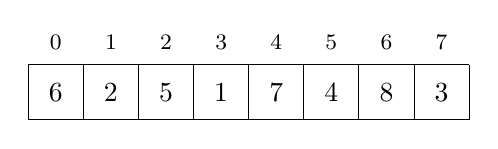
\begin{tikzpicture}[scale=0.7]
\draw (0,0) grid (8,1);
\node at (0.5,0.5) {$6$};
\node at (1.5,0.5) {$2$};
\node at (2.5,0.5) {$5$};
\node at (3.5,0.5) {$1$};
\node at (4.5,0.5) {$7$};
\node at (5.5,0.5) {$4$};
\node at (6.5,0.5) {$8$};
\node at (7.5,0.5) {$3$};

\footnotesize
\node at (0.5,1.4) {$0$};
\node at (1.5,1.4) {$1$};
\node at (2.5,1.4) {$2$};
\node at (3.5,1.4) {$3$};
\node at (4.5,1.4) {$4$};
\node at (5.5,1.4) {$5$};
\node at (6.5,1.4) {$6$};
\node at (7.5,1.4) {$7$};
\end{tikzpicture}
\end{center}
طولانی‌ترین زیردنباله صعودی شامل ۴ عنصر است:
\begin{center}
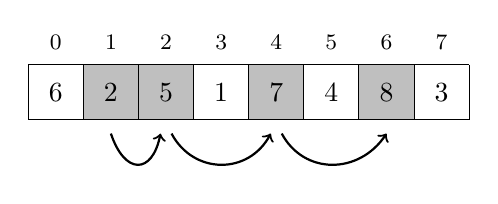
\begin{tikzpicture}[scale=0.7]
\fill[color=lightgray] (1,0) rectangle (2,1);
\fill[color=lightgray] (2,0) rectangle (3,1);
\fill[color=lightgray] (4,0) rectangle (5,1);
\fill[color=lightgray] (6,0) rectangle (7,1);
\draw (0,0) grid (8,1);
\node at (0.5,0.5) {$6$};
\node at (1.5,0.5) {$2$};
\node at (2.5,0.5) {$5$};
\node at (3.5,0.5) {$1$};
\node at (4.5,0.5) {$7$};
\node at (5.5,0.5) {$4$};
\node at (6.5,0.5) {$8$};
\node at (7.5,0.5) {$3$};

\draw[thick,->] (1.5,-0.25) .. controls (1.75,-1.00) and (2.25,-1.00) .. (2.4,-0.25);
\draw[thick,->] (2.6,-0.25) .. controls (3.0,-1.00) and (4.0,-1.00) .. (4.4,-0.25);
\draw[thick,->] (4.6,-0.25) .. controls (5.0,-1.00) and (6.0,-1.00) .. (6.5,-0.25);

\footnotesize
\node at (0.5,1.4) {$0$};
\node at (1.5,1.4) {$1$};
\node at (2.5,1.4) {$2$};
\node at (3.5,1.4) {$3$};
\node at (4.5,1.4) {$4$};
\node at (5.5,1.4) {$5$};
\node at (6.5,1.4) {$6$};
\node at (7.5,1.4) {$7$};
\end{tikzpicture}
\end{center}

فرض کنید $\texttt{length}(k)$ نشان‌دهنده طول طولانی‌ترین زیردنباله صعودی باشد که در موقعیت $k$ خاتمه می‌یابد.
بنابراین، اگر تمام مقادیر $\texttt{length}(k)$ را به ازای $0 \le k \le n-1$ محاسبه کنیم، طول طولانی‌ترین زیردنباله صعودی را به دست خواهیم آورد.
برای مثال، مقادیر تابع برای آرایه فوق به شرح زیر است:
\[
\begin{array}{lcl}
\texttt{length}(0) & = & 1 \\
\texttt{length}(1) & = & 1 \\
\texttt{length}(2) & = & 2 \\
\texttt{length}(3) & = & 1 \\
\texttt{length}(4) & = & 3 \\
\texttt{length}(5) & = & 2 \\
\texttt{length}(6) & = & 4 \\
\texttt{length}(7) & = & 2 \\
\end{array}
\]

برای نمونه، $\texttt{length}(6)=4$ است، زیرا طولانی‌ترین زیردنباله صعودی منتهی به موقعیت ۶ متشکل از ۴ عنصر است.

جهت محاسبه مقدار $\texttt{length}(k)$، باید موقعیتی مانند $i<k$ بیابیم که در آن $\texttt{array}[i]<\texttt{array}[k]$ باشد و $\texttt{length}(i)$ بیشترین مقدار ممکن را داشته باشد.
سپس می‌دانیم که $\texttt{length}(k)=\texttt{length}(i)+1$ خواهد بود، زیرا این روش بهینه برای افزودن $\texttt{array}[k]$ به یک زیردنباله است.
اما اگر چنین موقعیتی مانند $i$ وجود نداشته باشد، آنگاه $\texttt{length}(k)=1$ می‌شود، به این معنی که زیردنباله تنها شامل $\texttt{array}[k]$ است.

از آنجا که تمام مقادیر تابع از روی مقادیر کوچک‌تر آن قابل محاسبه است، می‌توان از برنامه‌نویسی پویا بهره برد.
در کد زیر، مقادیر تابع درون آرایه‌ای به نام $\texttt{length}$ ذخیره خواهد شد.

\begin{lstlisting}
for (int k = 0; k < n; k++) {
    length[k] = 1;
    for (int i = 0; i < k; i++) {
        if (array[i] < array[k]) {
            length[k] = max(length[k],length[i]+1);
        }
    }
}
\end{lstlisting}

این کد در زمان $O(n^2)$ اجرا می‌شود،
زیرا شامل دو حلقه تو‌در‌تو است.
با این حال، می‌توان محاسبات برنامه‌نویسی پویا را
به شکل کارآمدتری در زمان $O(n \log n)$ نیز پیاده‌سازی کرد.
آیا می‌توانید روشی برای این کار بیابید؟

\section{مسیرها در جدول}

مسئله بعدی یافتن مسیری از گوشه بالا-چپ
به گوشه پایین-راست در یک جدول $n \times n$ است،
به‌طوری‌که تنها مجاز به حرکت به سمت پایین و راست باشیم.
هر خانه شامل یک عدد صحیح مثبت است
و مسیر باید به گونه‌ای انتخاب شود که
مجموع مقادیر در طول مسیر بیشترین مقدار ممکن باشد.

تصویر زیر یک مسیر بهینه را در جدول نشان می‌دهد:
\begin{center}
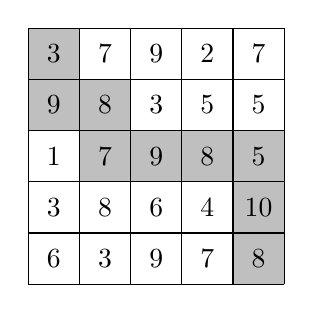
\begin{tikzpicture}[scale=.65]
  \begin{scope}
    \fill [color=lightgray] (0, 9) rectangle (1, 8);
    \fill [color=lightgray] (0, 8) rectangle (1, 7);
    \fill [color=lightgray] (1, 8) rectangle (2, 7);
    \fill [color=lightgray] (1, 7) rectangle (2, 6);
    \fill [color=lightgray] (2, 7) rectangle (3, 6);
    \fill [color=lightgray] (3, 7) rectangle (4, 6);
    \fill [color=lightgray] (4, 7) rectangle (5, 6);
    \fill [color=lightgray] (4, 6) rectangle (5, 5);
    \fill [color=lightgray] (4, 5) rectangle (5, 4);
    \draw (0, 4) grid (5, 9);
    \node at (0.5,8.5) {3};
    \node at (1.5,8.5) {7};
    \node at (2.5,8.5) {9};
    \node at (3.5,8.5) {2};
    \node at (4.5,8.5) {7};
    \node at (0.5,7.5) {9};
    \node at (1.5,7.5) {8};
    \node at (2.5,7.5) {3};
    \node at (3.5,7.5) {5};
    \node at (4.5,7.5) {5};
    \node at (0.5,6.5) {1};
    \node at (1.5,6.5) {7};
    \node at (2.5,6.5) {9};
    \node at (3.5,6.5) {8};
    \node at (4.5,6.5) {5};
    \node at (0.5,5.5) {3};
    \node at (1.5,5.5) {8};
    \node at (2.5,5.5) {6};
    \node at (3.5,5.5) {4};
    \node at (4.5,5.5) {10};
    \node at (0.5,4.5) {6};
    \node at (1.5,4.5) {3};
    \node at (2.5,4.5) {9};
    \node at (3.5,4.5) {7};
    \node at (4.5,4.5) {8};
  \end{scope}
\end{tikzpicture}
\end{center}
مجموع مقادیر در این مسیر برابر ۶۷ است
و این بیشترین مجموع ممکن برای مسیری از
گوشه بالا-چپ به گوشه پایین-راست می‌باشد.

فرض کنید سطرها و ستون‌های جدول
از ۱ تا $n$ شماره‌گذاری شده‌اند
و $\texttt{value}[y][x]$ برابر با مقدار خانه $(y,x)$ است.
فرض کنید $\texttt{sum}(y,x)$ بیشترین مجموع
در مسیری از گوشه بالا-چپ به خانه $(y,x)$ را نشان دهد.
در این صورت $\texttt{sum}(n,n)$ بیشترین مجموع
از گوشه بالا-چپ تا گوشه پایین-راست را مشخص می‌کند.
برای نمونه، در جدول بالا داریم:
$\texttt{sum}(5,5)=67$.

می‌توان مجموع‌ها را به صورت بازگشتی
به شکل زیر محاسبه کرد:
\[ \texttt{sum}(y,x) = \max(\texttt{sum}(y,x-1),\texttt{sum}(y-1,x))+\texttt{value}[y][x]\]

فرمول بازگشتی مبتنی بر این مشاهده است
که مسیر منتهی به خانه $(y,x)$
فقط می‌تواند از خانه $(y,x-1)$
یا از خانه $(y-1,x)$ بیاید:
\begin{center}
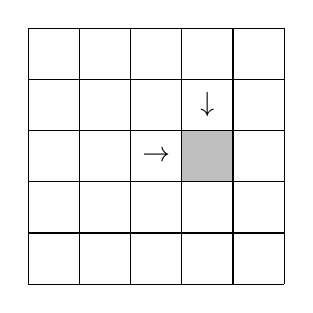
\begin{tikzpicture}[scale=.65]
  \begin{scope}
    \fill [color=lightgray] (3, 7) rectangle (4, 6);
    \draw (0, 4) grid (5, 9);
    
    \node at (2.5,6.5) {$\rightarrow$};
    \node at (3.5,7.5) {$\downarrow$};
    
  \end{scope}
\end{tikzpicture}
\end{center}

بنابراین، جهتی انتخاب می‌شود که مجموع را بیشینه کند.
فرض می‌شود $\texttt{sum}(y,x)=0$
اگر $y=0$ یا $x=0$ باشد (چون چنین مسیری وجود ندارد)،
بنابراین فرمول بازگشتی برای $y=1$ یا $x=1$ نیز کار می‌کند.

چون تابع \texttt{sum} دو پارامتر دارد،
آرایه برنامه‌نویسی پویا نیز دو بعدی است.
برای مثال، می‌توان از آرایه زیر استفاده کرد:
\begin{lstlisting}
int sum[N][N];
\end{lstlisting}
و مجموع‌ها را به این صورت محاسبه کرد:
\begin{lstlisting}
for (int y = 1; y <= n; y++) {
    for (int x = 1; x <= n; x++) {
        sum[y][x] = max(sum[y][x-1],sum[y-1][x])+value[y][x];
    }
}
\end{lstlisting}
پیچیدگی زمانی الگوریتم $O(n^2)$ است.

\section{مسائل کوله‌پشتی}

\index{knapsack}

اصطلاح \key{کوله‌پشتی} به مسائلی اشاره دارد که
مجموعه‌ای از اشیاء داده شده و
باید زیرمجموعه‌هایی با ویژگی‌های مشخص پیدا شوند.
مسائل کوله‌پشتی اغلب با برنامه‌نویسی پویا حل می‌شوند.

در این بخش، تمرکز روی این مسئله است:
به ازای فهرستی از وزن‌ها
$[w_1,w_2,\ldots,w_n]$،
تمام مجموع‌هایی که می‌توان با این وزن‌ها ساخت مشخص شوند.
برای مثال، اگر وزن‌ها
$[1,3,3,5]$ باشند، این مجموع‌ها ممکن هستند:

\begin{center}
\begin{tabular}{rrrrrrrrrrrrr}
 0 & 1 & 2 & 3 & 4 & 5 & 6 & 7 & 8 & 9 & 10 & 11 & 12 \\
\hline
 X & X & & X & X & X & X & X & X & X & & X & X \\
\end{tabular}
\end{center}

در این حالت، تمام مجموع‌های بین $0 \ldots 12$
به جز 2 و 10 ممکن هستند.
برای مثال، مجموع 7 ممکن است چون می‌توان
وزن‌های $[1,3,3]$ را انتخاب کرد.

برای حل مسئله، تمرکز روی زیرمسائلی است
که فقط از $k$ وزن اول برای ساخت مجموع‌ها استفاده می‌کنند.
فرض کنید $\texttt{possible}(x,k)=\textrm{true}$ باشد اگر
بتوان مجموع $x$ را با استفاده از $k$ وزن اول ساخت،
و در غیر این صورت $\texttt{possible}(x,k)=\textrm{false}$.
مقادیر تابع به صورت بازگشتی این‌گونه محاسبه می‌شوند:
\[ \texttt{possible}(x,k) = \texttt{possible}(x-w_k,k-1) \lor \texttt{possible}(x,k-1) \]
فرمول بر این اساس است که وزن $w_k$ در مجموع استفاده شود یا نشود.
اگر $w_k$ استفاده شود، کار باقی‌مانده ساخت مجموع $x-w_k$ با $k-1$ وزن اول است،
و اگر $w_k$ استفاده نشود،
کار باقی‌مانده ساخت مجموع $x$ با $k-1$ وزن اول است.
به عنوان حالت‌های پایه:
\begin{equation*}
    \texttt{possible}(x,0) = \begin{cases}
               \textrm{true}    & x = 0\\
               \textrm{false}   & x \neq 0 \\
           \end{cases}
\end{equation*}
چون اگر هیچ وزنی استفاده نشود،
فقط مجموع 0 قابل ساخت است.

جدول زیر همه مقادیر تابع را برای وزن‌های $[1,3,3,5]$ نشان می‌دهد (علامت ''X'' نشان‌دهنده مقادیر درست است):

\begin{center}
\begin{tabular}{r|rrrrrrrrrrrrr}
$k \backslash x$ & 0 & 1 & 2 & 3 & 4 & 5 & 6 & 7 & 8 & 9 & 10 & 11 & 12 \\
\hline
 0 & X & \\
 1 & X & X \\
 2 & X & X & & X & X \\
 3 & X & X & & X & X & & X & X \\
 4 & X & X & & X & X & X & X & X & X & X & & X & X \\
\end{tabular}
\end{center}

پس از محاسبه این مقادیر، $\texttt{possible}(x,n)$ مشخص می‌کند آیا می‌توان با استفاده از \emph{همه} وزن‌ها به مجموع $x$ رسید یا خیر.

فرض کنید $W$ مجموع کل وزن‌ها باشد. راه‌حل برنامه‌نویسی پویا زیر با پیچیدگی زمانی $O(nW)$ متناظر با تابع بازگشتی است:
\begin{lstlisting}
possible[0][0] = true;
for (int k = 1; k <= n; k++) {
    for (int x = 0; x <= W; x++) {
        if (x-w[k] >= 0) possible[x][k] |= possible[x-w[k]][k-1];
        possible[x][k] |= possible[x][k-1];
    }
}
\end{lstlisting}

با این حال، پیاده‌سازی بهتری وجود دارد که تنها از یک آرایه یک‌بعدی $\texttt{possible}[x]$ استفاده می‌کند؛ آرایه‌ای که مشخص می‌سازد آیا ساخت زیرمجموعه‌ای با مجموع $x$ ممکن است یا خیر. ترفند کار، به‌روزرسانی آرایه از راست به چپ برای هر وزن جدید است:
\begin{lstlisting}
possible[0] = true;
for (int k = 1; k <= n; k++) {
    for (int x = W; x >= 0; x--) {
        if (possible[x]) possible[x+w[k]] = true;
    }
}
\end{lstlisting}

توجه داشته باشید که ایده کلی ارائه‌شده در اینجا در بسیاری از مسائل کوله‌پشتی کاربرد دارد. به عنوان مثال، اگر اشیایی با وزن‌ها و ارزش‌های مشخص داده شوند، می‌توانیم به ازای هر مجموع وزن، بیشترین مجموع ارزش یک زیرمجموعه را تعیین کنیم.

\section{فاصله ویرایشی}

\index{فاصله ویرایشی}
\index{فاصله لون‌اشتاین}

\key{فاصله ویرایشی} یا \key{فاصله لون‌اشتاین}\footnote{این فاصله به نام وی. آی. لون‌اشتاین نام‌گذاری شده است که آن را در ارتباط با کدهای دودویی بررسی کرد \cite{lev66}.} کمینه تعداد عملیات‌های ویرایشی مورد نیاز برای تبدیل یک رشته به رشته‌ای دیگر است. عملیات‌های ویرایشی مجاز عبارتند از:
\begin{itemize}
\item درج یک نویسه (مثال: \texttt{ABC} $\rightarrow$ \texttt{ABCA})
\item حذف یک نویسه (مثال: \texttt{ABC} $\rightarrow$ \texttt{AC})
\item تغییر یک نویسه (مثال: \texttt{ABC} $\rightarrow$ \texttt{ADC})
\end{itemize}

برای نمونه، فاصله ویرایشی بین \texttt{LOVE} و \texttt{MOVIE} برابر ۲ است، زیرا ابتدا می‌توان عملیات \texttt{LOVE} $\rightarrow$ \texttt{MOVE} (تغییر) و سپس عملیات \texttt{MOVE} $\rightarrow$ \texttt{MOVIE} (درج) را انجام داد. این کمترین تعداد عملیات ممکن است، زیرا مشخص است که تنها یک عملیات کافی نیست.

فرض کنید رشته \texttt{x} با طول $n$ و رشته \texttt{y} با طول $m$ داده شده‌اند
و هدف، محاسبه فاصله ویرایشی بین \texttt{x} و \texttt{y} است.
برای حل مسئله، تابع $\texttt{distance}(a,b)$ را تعریف می‌کنیم
که فاصله ویرایشی بین پیشوندهای $\texttt{x}[0 \ldots a]$ و $\texttt{y}[0 \ldots b]$ را می‌دهد.
بنابراین با استفاده از این تابع، فاصله ویرایشی
بین \texttt{x} و \texttt{y} برابر با $\texttt{distance}(n-1,m-1)$ است.

مقادیر \texttt{distance} را می‌توان به این صورت محاسبه کرد:
\begin{equation*}
\begin{split}
\texttt{distance}(a,b) = \min(& \texttt{distance}(a,b-1)+1, \\
                           & \texttt{distance}(a-1,b)+1, \\
                           & \texttt{distance}(a-1,b-1)+\texttt{cost}(a,b)).
\end{split}
\end{equation*}
در اینجا اگر $\texttt{x}[a]=\texttt{y}[b]$ باشد مقدار $\texttt{cost}(a,b)=0$،
و در غیر این صورت $\texttt{cost}(a,b)=1$ است.
این رابطه حالات زیر را برای ویرایش رشته \texttt{x} در نظر می‌گیرد:
\begin{itemize}
\item $\texttt{distance}(a,b-1)$: درج یک نویسه در انتهای \texttt{x}
\item $\texttt{distance}(a-1,b)$: حذف آخرین نویسه از \texttt{x}
\item $\texttt{distance}(a-1,b-1)$: تطابق یا تغییر آخرین نویسه \texttt{x}
\end{itemize}
در دو حالت اول، یک عملیات ویرایش نیاز است
(درج یا حذف).
در حالت آخر، اگر $\texttt{x}[a]=\texttt{y}[b]$ باشد،
می‌توان آخرین نویسه‌ها را بدون ویرایش تطابق داد،
و در غیر این صورت یک عملیات ویرایش نیاز است (تغییر).

جدول زیر مقادیر \texttt{distance} را در مثال نمونه نشان می‌دهد:
\begin{center}
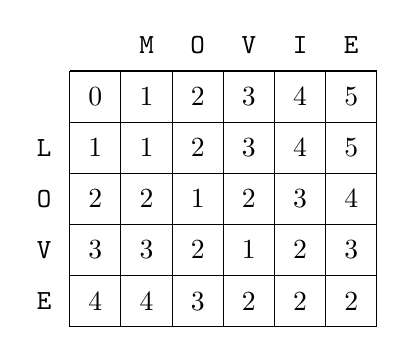
\begin{tikzpicture}[scale=.65]
  \begin{scope}
    %\fill [color=lightgray] (5, -3) rectangle (6, -4);
    \draw (1, -1) grid (7, -6);
    
    \node at (0.5,-2.5) {\texttt{L}};
    \node at (0.5,-3.5) {\texttt{O}};
    \node at (0.5,-4.5) {\texttt{V}};
    \node at (0.5,-5.5) {\texttt{E}};

    \node at (2.5,-0.5) {\texttt{M}};
    \node at (3.5,-0.5) {\texttt{O}};
    \node at (4.5,-0.5) {\texttt{V}};
    \node at (5.5,-0.5) {\texttt{I}};
    \node at (6.5,-0.5) {\texttt{E}};

    \node at (1.5,-1.5) {$0$};
    \node at (1.5,-2.5) {$1$};
    \node at (1.5,-3.5) {$2$};
    \node at (1.5,-4.5) {$3$};
    \node at (1.5,-5.5) {$4$};
    \node at (2.5,-1.5) {$1$};
    \node at (2.5,-2.5) {$1$};
    \node at (2.5,-3.5) {$2$};
    \node at (2.5,-4.5) {$3$};
    \node at (2.5,-5.5) {$4$};
    \node at (3.5,-1.5) {$2$};
    \node at (3.5,-2.5) {$2$};
    \node at (3.5,-3.5) {$1$};
    \node at (3.5,-4.5) {$2$};
    \node at (3.5,-5.5) {$3$};
    \node at (4.5,-1.5) {$3$};
    \node at (4.5,-2.5) {$3$};
    \node at (4.5,-3.5) {$2$};
    \node at (4.5,-4.5) {$1$};
    \node at (4.5,-5.5) {$2$};
    \node at (5.5,-1.5) {$4$};
    \node at (5.5,-2.5) {$4$};
    \node at (5.5,-3.5) {$3$};
    \node at (5.5,-4.5) {$2$};
    \node at (5.5,-5.5) {$2$};
    \node at (6.5,-1.5) {$5$};
    \node at (6.5,-2.5) {$5$};
    \node at (6.5,-3.5) {$4$};
    \node at (6.5,-4.5) {$3$};
    \node at (6.5,-5.5) {$2$};
  \end{scope}
\end{tikzpicture}
\end{center}

گوشه پایین و راست جدول
نشان می‌دهد فاصله ویرایشی بین
\texttt{LOVE} و \texttt{MOVIE} برابر ۲ است.
همچنین، جدول نحوه ساخت
کوتاه‌ترین دنباله از عملیات ویرایشی را نشان می‌دهد.
در این حالت، مسیر به صورت زیر است:

\begin{center}
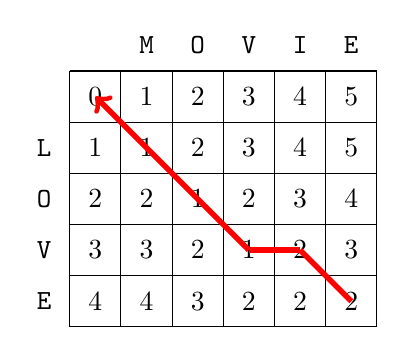
\begin{tikzpicture}[scale=.65]
  \begin{scope}
    \draw (1, -1) grid (7, -6);
    
    \node at (0.5,-2.5) {\texttt{L}};
    \node at (0.5,-3.5) {\texttt{O}};
    \node at (0.5,-4.5) {\texttt{V}};
    \node at (0.5,-5.5) {\texttt{E}};

    \node at (2.5,-0.5) {\texttt{M}};
    \node at (3.5,-0.5) {\texttt{O}};
    \node at (4.5,-0.5) {\texttt{V}};
    \node at (5.5,-0.5) {\texttt{I}};
    \node at (6.5,-0.5) {\texttt{E}};

    \node at (1.5,-1.5) {$0$};
    \node at (1.5,-2.5) {$1$};
    \node at (1.5,-3.5) {$2$};
    \node at (1.5,-4.5) {$3$};
    \node at (1.5,-5.5) {$4$};
    \node at (2.5,-1.5) {$1$};
    \node at (2.5,-2.5) {$1$};
    \node at (2.5,-3.5) {$2$};
    \node at (2.5,-4.5) {$3$};
    \node at (2.5,-5.5) {$4$};
    \node at (3.5,-1.5) {$2$};
    \node at (3.5,-2.5) {$2$};
    \node at (3.5,-3.5) {$1$};
    \node at (3.5,-4.5) {$2$};
    \node at (3.5,-5.5) {$3$};
    \node at (4.5,-1.5) {$3$};
    \node at (4.5,-2.5) {$3$};
    \node at (4.5,-3.5) {$2$};
    \node at (4.5,-4.5) {$1$};
    \node at (4.5,-5.5) {$2$};
    \node at (5.5,-1.5) {$4$};
    \node at (5.5,-2.5) {$4$};
    \node at (5.5,-3.5) {$3$};
    \node at (5.5,-4.5) {$2$};
    \node at (5.5,-5.5) {$2$};
    \node at (6.5,-1.5) {$5$};
    \node at (6.5,-2.5) {$5$};
    \node at (6.5,-3.5) {$4$};
    \node at (6.5,-4.5) {$3$};
    \node at (6.5,-5.5) {$2$};

    \path[draw=red,thick,-,line width=2pt] (6.5,-5.5) -- (5.5,-4.5);
    \path[draw=red,thick,-,line width=2pt] (5.5,-4.5) -- (4.5,-4.5);
    \path[draw=red,thick,->,line width=2pt] (4.5,-4.5) -- (1.5,-1.5);
  \end{scope}
\end{tikzpicture}
\end{center}

نویسه‌های آخر \texttt{LOVE} و \texttt{MOVIE}
برابرند، بنابراین فاصله ویرایشی بین آن‌ها
برابر با فاصله ویرایشی بین \texttt{LOV} و \texttt{MOVI} است.
می‌توان با یک عمل ویرایشی نویسه \texttt{I} را
از \texttt{MOVI} حذف کرد.
در نتیجه، فاصله ویرایشی یک واحد بیشتر از
فاصله ویرایشی بین \texttt{LOV} و \texttt{MOV} است و به همین ترتیب.

\section{شمارش کاشی‌کاری‌ها}

گاهی حالت‌های یک راهکار برنامه‌نویسی پویا
پیچیده‌تر از ترکیب‌های ثابتی از اعداد هستند.
به‌عنوان مثال، مسئله محاسبه تعداد روش‌های متمایز برای
پر کردن یک جدول $n \times m$ با استفاده از
کاشی‌های با ابعاد $1 \times 2$ و $2 \times 1$ را در نظر بگیرید.
به‌عنوان نمونه، یک جواب معتبر
برای جدول $4 \times 7$ عبارت است از:
\begin{center}
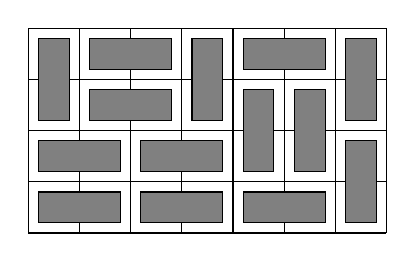
\begin{tikzpicture}[scale=.65]
    \draw (0,0) grid (7,4);
    \draw[fill=gray] (0+0.2,0+0.2) rectangle (2-0.2,1-0.2);
    \draw[fill=gray] (2+0.2,0+0.2) rectangle (4-0.2,1-0.2);
    \draw[fill=gray] (4+0.2,0+0.2) rectangle (6-0.2,1-0.2);
    \draw[fill=gray] (0+0.2,1+0.2) rectangle (2-0.2,2-0.2);
    \draw[fill=gray] (2+0.2,1+0.2) rectangle (4-0.2,2-0.2);
    \draw[fill=gray] (1+0.2,2+0.2) rectangle (3-0.2,3-0.2);
    \draw[fill=gray] (1+0.2,3+0.2) rectangle (3-0.2,4-0.2);
    \draw[fill=gray] (4+0.2,3+0.2) rectangle (6-0.2,4-0.2);

    \draw[fill=gray] (0+0.2,2+0.2) rectangle (1-0.2,4-0.2);
    \draw[fill=gray] (3+0.2,2+0.2) rectangle (4-0.2,4-0.2);
    \draw[fill=gray] (6+0.2,2+0.2) rectangle (7-0.2,4-0.2);
    \draw[fill=gray] (4+0.2,1+0.2) rectangle (5-0.2,3-0.2);
    \draw[fill=gray] (5+0.2,1+0.2) rectangle (6-0.2,3-0.2);
    \draw[fill=gray] (6+0.2,0+0.2) rectangle (7-0.2,2-0.2);

\end{tikzpicture}
\end{center}
و تعداد کل جواب‌ها برابر ۷۸۱ است.

این مسئله را می‌توان با برنامه‌نویسی پویا
و با پیمایش سطر به سطر جدول حل کرد.
هر سطر در یک جواب را می‌توان به‌صورت رشته‌ای
شامل $m$ نویسه از مجموعه
$\{\sqcap, \sqcup, \sqsubset, \sqsupset \}$ نشان داد.
برای مثال، جواب بالا شامل چهار سطر است
که متناظر با رشته‌های زیر هستند:
\begin{itemize}
\item
$\sqcap \sqsubset \sqsupset \sqcap \sqsubset \sqsupset \sqcap$
\item
$\sqcup \sqsubset \sqsupset \sqcup \sqcap \sqcap \sqcup$
\item
$\sqsubset \sqsupset \sqsubset \sqsupset \sqcup \sqcup \sqcap$ 
\item
$\sqsubset \sqsupset \sqsubset \sqsupset \sqsubset \sqsupset \sqcup$
\end{itemize}

فرض کنید $\texttt{count}(k,x)$ بیانگر تعداد روش‌های
ساخت یک جواب برای سطرهای $1 \ldots k$
از جدول باشد به‌طوری که رشته $x$ متناظر با سطر $k$ باشد.
استفاده از برنامه‌نویسی پویا در اینجا ممکن است،
زیرا وضعیت یک سطر فقط توسط
وضعیت سطر قبلی محدود می‌شود.

یک پاسخ معتبر است اگر سطر $1$ شامل نویسه $\sqcup$ نباشد، سطر $n$ شامل نویسه $\sqcap$ نباشد، و تمام سطرهای متوالی \emph{سازگار} باشند.
برای نمونه، سطرهای
$\sqcup \sqsubset \sqsupset \sqcup \sqcap \sqcap \sqcup$ و
$\sqsubset \sqsupset \sqsubset \sqsupset \sqcup \sqcup \sqcap$ 
سازگارند، در حالی که سطرهای
$\sqcap \sqsubset \sqsupset \sqcap \sqsubset \sqsupset \sqcap$ و
$\sqsubset \sqsupset \sqsubset \sqsupset \sqsubset \sqsupset \sqcup$
سازگار نیستند.

چون هر سطر شامل $m$ نویسه است و برای هر نویسه چهار انتخاب وجود دارد، تعداد سطرهای متمایز حداکثر $4^m$ است.
بنابراین، پیچیدگی زمانی راه حل $O(n 4^{2m})$ است؛ چون برای هر سطر می‌توان $O(4^m)$ حالت ممکن را پیمایش کرد، و برای هر حالت، $O(4^m)$ حالت ممکن برای سطر قبلی وجود دارد.
در عمل، بهتر است جدول چرخ Mel شود تا ضلع کوتاه‌تر طول $m$ داشته باشد، زیرا ضریب $4^{2m}$ بر پیچیدگی زمانی غالب است.

می‌توان با استفاده از نمایش فشرده‌تر برای سطرها، کارایی راه حل را افزایش داد.
مشخص می‌شود کافی است بدانیم کدام ستون‌های سطر قبل شامل مربع بالایی یک کاشی عمودی هستند.
بنابراین، می‌توان یک سطر را تنها با استفاده از نویسه‌های $\sqcap$ و $\Box$ نشان داد، که در آن $\Box$ ترکیبی از نویسه‌های $\sqcup$، $\sqsubset$ و $\sqsupset$ است.
با استفاده از این نمایش، تنها $2^m$ سطر متمایز وجود دارد و پیچیدگی زمانی $O(n 2^{2m})$ خواهد بود.

به عنوان نکته پایانی، یک فرمول مستقیم شگفت‌انگیز نیز برای محاسبه تعداد کاشی‌کاری‌ها وجود دارد\footnote{به طرز شگفت‌آوری، این فرمول در سال ۱۹۶۱ توسط دو تیم پژوهشی \cite{kas61,tem61} که به طور مستقل کار می‌کردند کشف شد.}:
\[ \prod_{a=1}^{\lceil n/2 \rceil} \prod_{b=1}^{\lceil m/2 \rceil} 4 \cdot (\cos^2 \frac{\pi a}{n + 1} + \cos^2 \frac{\pi b}{m+1})\]
این فرمول بسیار کارآمد است، زیرا تعداد کاشی‌کاری‌ها را در زمان $O(nm)$ محاسبه می‌کند، اما چون پاسخ حاصل‌ضرب اعداد حقیقی است، چالش هنگام استفاده از فرمول، ذخیره دقیق نتایج میانی است.